\section[Aktivační měření, gama spektroskopie]{Neutronová pole pro aktivační analýzu, fyzikální principy aktivačních měření, využití gama spektroskopie}

\subsection{Zdroje neutronů}

\subsubsection{Radionuklidové zdroje}

\textbf{Spontánní štěpení:} u některých transuranů existuje nenulová pravděpodobnost, že mimo tradiční rozpady podléhají spontánnímu štěpení. Typickým příkladem je $^{252}$Cf s $T_{1/2} = 2,6$ let a s $\nu = 3,75$ (3,1 \% štěpení, zbytek $\alpha$). Výsledkem je spojité spektrum v oblasti rychlých neutronů (střední energie 2,1 MeV) dle Wattovy distribuce:

$$ \chi(E) = A e^{B E_n} \: \text{sinh} (C \cdot E_n). $$

Emisivita komerčních zdrojů se pohybuje řádově 10$^9$ až 10$^{10}$ 1/s, prodává se ve formě zapouzdřeného oxidu CfO$_2$.

\textbf{($\alpha$,n) reakce:} jde o prahovou reakci na vybraných izotopech, primárně $^9$Be. V tomto důsledku vzniká i doprovodné gamma záření (4,4 MeV pro $^9$Be).

K tomu se přidá $\alpha$ zářič, který emituje primární $\alpha$ částice, a ty vyrážejí sekundární neutrony. Primární zářič se vybírá v závislosti na poločasu rozpadu (ten určuje emisivitu) a doprovodného gamma záření. Jde primárně o $^{210}$Po (poločas 138 dní), $^{238}$Pu (poločas 70 let, skoro žádná gamma), $^{241}$Am (poločas 400 let).

Výsledkem je opět spojité záření (kvůli proměnné energii primární $\alpha$ částice) v rychlé oblasti neutronů. Ve fromě oxidů PoBe, AmBe, PuBe apod. Komerční emisivita 10$^5$ až 10$^9$ 1/s.

\begin{figure}[H]
    \centering
    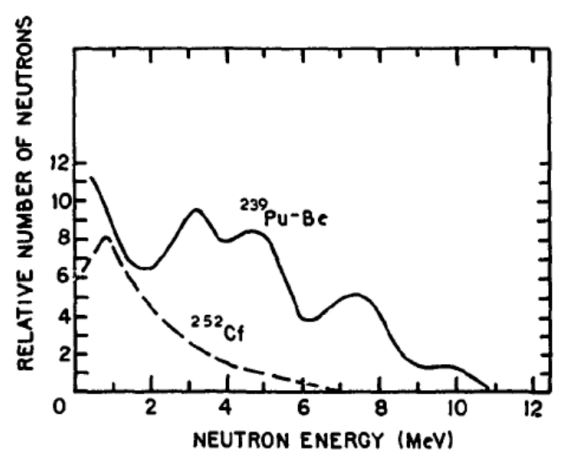
\includegraphics[width=0.4\textwidth]{img/zdroje_E.JPG}
    \caption{Srovnání emitovaného neutronového spektra pro spontánní štěpení a ($\alpha$,n) reakce.}
\end{figure}

\textbf{($\gamma$,n) reakce:} obdobné, opět prahové reakce na vybraných izotopech, primárně $^9$Be (1,67 MeV), $^2$H (2,23 MeV).

Vyžaduje vysokoenergetický gamma zářič ($^{24}$Na, $^{28}$Al, $^{38}$Cl, $^{56}$Mn, $^{226}$Ra). Opět intenzita ovlivněna poločasem rozpadu primárního zářiče.

Výhodou je, že pokud máme monoenergetický primární zářič (není více linek), tak vznikají monoenergetické neutrony. Nevýhoda je, že mají nižší výtěžek a pro vyšší emisivitu (řádově 10$^5$ 1/s) je zapotřebí velmi silné gamma zářiče.

\subsubsection{Zbylé zdroje}

\textbf{Jaderné reaktory:} nejintenzivnější zdroje neutronů, spektrum v závislosti na typu reaktoru, moderace apod. Je možné vytvářet kolimované svazky (radiální kanál + kolimátor (trubka)) o intenzitách 10$^{10}$ 1/s. V pulzním režimu až o několik řádů více.

V případě moderovaných systémů se distribuce může popsat Wattovou formulí, 1/$E^x$ oblastí a Maxwellovým rozdělením.

Dále je možné aplikovat filtry a vytvářet kvazimonoenergetická spektra (Sc, Si, Fe, S apod.).

\textbf{Neutronové generátory:} založeny na prahových reakcích urychlených nabitých částic (D+D, D+T, T+T reakce). Vznikají spojitá spektra s rychlými neutrony o emisivitě až $10^{10}$ 1/s.

Mohou být kompaktní, jdou vypnout, fungují i v pulzním režimu.

\begin{figure}[H]
    \centering
    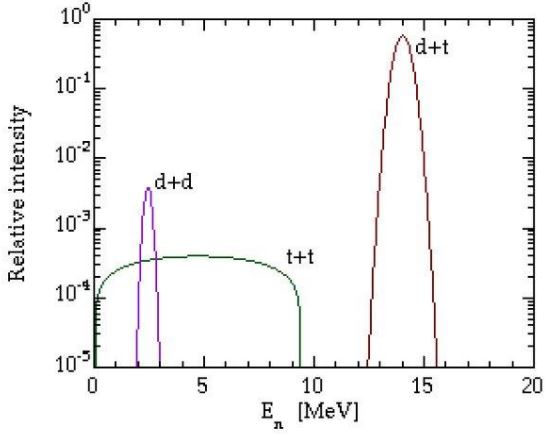
\includegraphics[width=0.4\textwidth]{img/generatory_E.JPG}
    \caption{Emitované spektrum pro neutronové generátory.}
\end{figure}

\textbf{Urychlovačem řízené zdroje:} stejný princip, pouze větší urychlovače, více typů reakcí (jenom změním terčík na $^7$Li, $^9$Be aj.) a mnohem větší emisivita.

Pro tenký terčík získáme čárové spektrum, pro tlustý terčík (před interakcí dojde ke zpomalení primárních částic) spojité spektrum. Využívá se pro výzkumné účely, hlavně pro aktivační měření.

\textbf{Spalačné zdroje:} pokud ještě více zvětším energii primárních částic (řádově GeVy), dojde k rozbití atomu na jednotlivé nukleony, což má za následek mnohem větší emisivitu. Jako terčík se využívají těžké prvky (W, U, Pb apod.). Vzniká široké spojité spektrum (vysokoenergetické, mohou vzniknout neutrony s energií desítek a stovek MeV).

\subsubsection{Zdroje pro aktivační měření}

Nejlepšími neutronovými zdroji pro aktivační měření jsou:

\begin{itemize}
    \item Výzkumné jaderné reaktory:
    \item[-] toky alepoň 10$^9$ 1/cm$^2$/s,
    \item[-] tepelné i epitermální neutrony, primárně (n,$\gamma$) reakce, kde jsou velké účinné průřezy, které jsou dobře proměřené,
    \item[-] případně možnost využít i prahové reakce (n,p), (n,2n) apod.
    \item Urychlovačem řízené zdroje:
    \item[-] toky alepoň 10$^10$ 1/cm$^2$/s,
    \item[-] využívají se reakce p + Be, d + Be
    \item[-] primárně rychlé neutrony ve spojitém spektru (tlustý terčík)
    \item[-] problém je, že v důsledku vícero prahových reakcí se otevírají nové kanály pro vznik daného izotopu. 
    \item Radionuklidové zdroje:
    \item[-] jsou přenositelné
    \item[-] mají menší emisivitu, proto se používají pouze u některých izotopů s vyšším účinným průřezem,
    \item[-] pro NAA jsou vhodné pouze za specifických podmínek. 
\end{itemize}

\subsection{Fyzikální principy aktivačních měření}

Veškeré aktivační měření jsou založeny na tom, že sleduju, které procesy se s daným vzorkem během ozařování v neutronovém procesu odehrály. Díky tomu je možné stanovit parametry neutronového pole, složení (kvantita i kvalita) aj.

\subsubsection{Reakční rychlost}

Vložím-li vzorek do neutronového pole, tak vzniká radioizotop $A$, který se rozpadá do izotopu $B$. Pokud ponecháme izotop v poli alespoň po dobu $10 \cdot T_A$, tak aktivita vzorku bude konvergovat k saturované aktivitě (produkce a destrukce izotopu $A$ je v rovnováze). 

\begin{figure}[H]
    \centering
    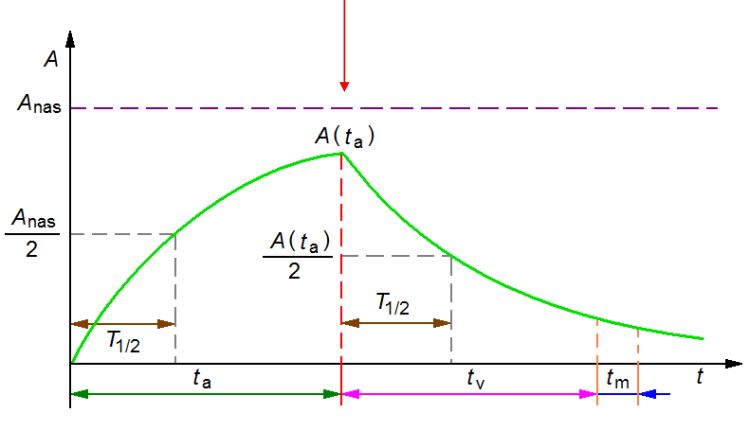
\includegraphics[width=0.6\textwidth]{img/saturovana_aktivita.JPG}
\end{figure}

Po jeho vyjmutí se začne rozpadat, přenese se do laboratoře a začíná se měřit jeho aktivita, ze které je možné zpětně dopočítat \textbf{reakční rychlost} $R$ (1/s), která stanovuje, ke kolika reakcím za jednotku času v daném neutronovém poli docházelo:

$$ \boxed{R = \int_{E_{min}}^{E_{max}} \phi(E) \sigma(E) \: \text{d}E = \dfrac{S \lambda \dfrac{t_\text{real}}{t_\text{live}}}{N_0 \: \varepsilon \: I \: (1-e^{-\lambda t_a}) \: e^{-\lambda t_v} \: (1-e^{-\lambda t_\text{real}}).}} $$

\begin{figure}[H]
    \centering
    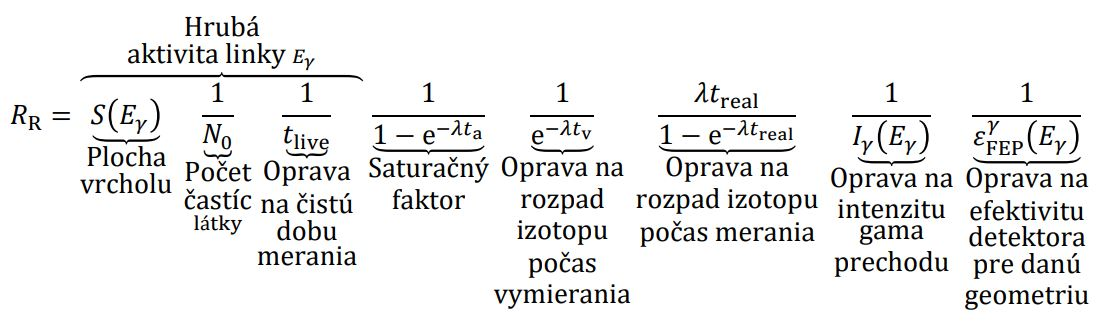
\includegraphics[width=0.8\textwidth]{img/RR_vyznam.JPG}
\end{figure}

Dále je třeba zahrnout vhodné opravné faktory (samostínění, nerovnoměrnost ozařování, geometrie, koincidenční sumační efekty apod.).

Pokud reakční rychlost pronásobím počtem atomů, získám \textbf{produkční rychlost} $R$ (1/s), tedy kolik se vyprodukuje nových izotopů za jednotku času:

$$ \boxed{ P = R \cdot N_0 = \dfrac{S \lambda \dfrac{t_\text{real}}{t_\text{live}}}{\varepsilon \: I \: (1-e^{-\lambda t_a}) \: e^{-\lambda t_v} \: (1-e^{-\lambda t_\text{real}})}.} $$

Pokud produkční rychlost pronásobím korekcí na vymírání, získám \textbf{aktivitu} $A$ (Bq) nově vzniklého izotopu:

$$ \boxed{ A = P \cdot e^{-\lambda t_v} = \dfrac{S \lambda \dfrac{t_\text{real}}{t_\text{live}}}{\varepsilon \: I \: (1-e^{-\lambda t_a}) \: (1-e^{-\lambda t_\text{real}})}.} $$

Navíc pokud skutečně vycházím ze saturované (nebo alespoň skorosaturované) aktivity, je možné vynechat i saturační faktor (je roven jedné), čímž získám stejnou rovnici z předešlé otázky:

$$ A = \dfrac{S \lambda \dfrac{t_\text{real}}{t_\text{live}}}{\varepsilon \: I \: (1-e^{-\lambda t_\text{real}}).} $$

\subsubsection{Generátorové rovnice}

Dále může docházet ke kaskádám, vznikne izotop $A$, který se rozpadá do $B$ a ten do $C$. Po chvíli dochází k rovnováhám mezi izotopy:

\begin{itemize}
    \item \textbf{Přechodná rovnováha} -- pokud $T_A > T_B$, k takovéto rovnováze dojde po uplynutí $10 \cdot T_B$, aktivity jsou v poměru:
    $$ \dfrac{A_B}{A_A} = \dfrac{T_A}{T_A - T_B}. $$
    \item \textbf{Dlouhodobá rovnováha} -- pokud $T_A >> T_B$, jde o limitní případ předešlého, kdy je $T_B$ zanedbatelně malý (okamžitý) a aktivity jsou v rovnováze:
    $$ A_A = A_B $$
    \item \textbf{Stav bez rovnováhy} -- pokud $T_A < T_B $, k rovnováze nedojde.
\end{itemize}

\subsubsection{Aplikace filtrů}

V neutronovém poli moderovaných jaderných reaktorů jsou neutrony o všech energiích, což je z hlediska aktivačního měření problematické (otevírají se nové reakční kanály, např. izotop $^{24}$Na může vzniknout za pomoci $^{23}$Na(n,$\gamma$)$^{24}$Na reakce v jakémkoliv spektru, nebo za pomoci $^{27}$Al(n,$\alpha$)$^{24}$Na v rychlém spektru). 

To je možné eliminovat za pomoci filtrů (kadmium), kdy odstraním efekt neutronů nad kadmiovou hranou. v závislosti na tom rozlišujeme:

\begin{itemize}
    \item ENNA = epitermální NNA,
    \item RNNA = reaktorová NAA.
\end{itemize}

Je možné využít i jiné filtry (B, Cl, Au, In, Al), ale musí být dostatečně tlusté, aby vykompenzovaly to, že nejsou tak dobrými absorbátory. Takto je možné odseparovat jednotlivé oblasti neutronového spektra.

\textbf{$^{113}$Cd} je vhodné pro energie pod 2 eV, nezahřívá se, stačí ho 1 mm, aktivované kadmium rychle vymírá. \textbf{$^{10}$B} je ideální nad 15 eV, nemá žádnou hranu, produkuje alfu, což vede k ohřevu vzorku. \textbf{Cd + B} je vhodné pro energie od 2 do 15 eV. 

\subsection{Využití gamma spektroskopie}